\documentclass[hidelinks,12pt]{article}
\usepackage[left=0.25cm,top=1cm,right=0.25cm,bottom=1cm]{geometry}
%\usepackage[landscape]{geometry}
\textwidth = 20cm
\hoffset = -1cm
\usepackage[utf8]{inputenc}
\usepackage[spanish,es-tabla]{babel}
\usepackage[autostyle,spanish=mexican]{csquotes}
\usepackage[tbtags]{amsmath}
\usepackage{nccmath}
\usepackage{amsthm}
\usepackage{amssymb}
\usepackage{mathrsfs}
\usepackage{graphicx}
\usepackage{subfig}
\usepackage{standalone}
\usepackage[outdir=./Imagenes/]{epstopdf}
\usepackage{siunitx}
\usepackage{physics}
\usepackage{color}
\usepackage{float}
\usepackage{hyperref}
\usepackage{multicol}
%\usepackage{milista}
\usepackage{anyfontsize}
\usepackage{anysize}
%\usepackage{enumerate}
\usepackage[shortlabels]{enumitem}
\usepackage{capt-of}
\usepackage{bm}
\usepackage{relsize}
\usepackage{placeins}
\usepackage{empheq}
\usepackage{cancel}
\usepackage{wrapfig}
\usepackage[flushleft]{threeparttable}
\usepackage{makecell}
\usepackage{fancyhdr}
\usepackage{tikz}
\usepackage{bigints}
\usepackage{scalerel}
\usepackage{pgfplots}
\usepackage{pdflscape}
\pgfplotsset{compat=1.16}
\spanishdecimal{.}
\renewcommand{\baselinestretch}{1.5} 
\renewcommand\labelenumii{\theenumi.{\arabic{enumii}})}
\newcommand{\ptilde}[1]{\ensuremath{{#1}^{\prime}}}
\newcommand{\stilde}[1]{\ensuremath{{#1}^{\prime \prime}}}
\newcommand{\ttilde}[1]{\ensuremath{{#1}^{\prime \prime \prime}}}
\newcommand{\ntilde}[2]{\ensuremath{{#1}^{(#2)}}}

\newtheorem{defi}{{\it Definición}}[section]
\newtheorem{teo}{{\it Teorema}}[section]
\newtheorem{ejemplo}{{\it Ejemplo}}[section]
\newtheorem{propiedad}{{\it Propiedad}}[section]
\newtheorem{lema}{{\it Lema}}[section]
\newtheorem{cor}{Corolario}
\newtheorem{ejer}{Ejercicio}[section]

\newlist{milista}{enumerate}{2}
\setlist[milista,1]{label=\arabic*)}
\setlist[milista,2]{label=\arabic{milistai}.\arabic*)}
\newlength{\depthofsumsign}
\setlength{\depthofsumsign}{\depthof{$\sum$}}
\newcommand{\nsum}[1][1.4]{% only for \displaystyle
    \mathop{%
        \raisebox
            {-#1\depthofsumsign+1\depthofsumsign}
            {\scalebox
                {#1}
                {$\displaystyle\sum$}%
            }
    }
}
\def\scaleint#1{\vcenter{\hbox{\scaleto[3ex]{\displaystyle\int}{#1}}}}
\def\bs{\mkern-12mu}


%\usepackage{showframe}
\usepackage{apacite}
\title{La función hipergeométrica \\ \large {Tema 5 - Funciones especiales} \vspace{-3ex}}
\author{M. en C. Gustavo Contreras Mayén}
\date{ }
\begin{document}
\vspace{-4cm}
\maketitle
\fontsize{14}{14}\selectfont
\tableofcontents
\newpage
%Referencia Riley 18.10 Hipergeometric functions
\section{Funciones hipergeométricas.}

La ecuación diferencial hipergeométrica tiene la forma:
\begin{align}
x (1 - x) \, \stilde{y} + \big[ c - (a + b - 1) \, x \big] \, \ptilde{y} -  a \, b \, y = 0
\label{eq:ecuacion_18_136}
\end{align}
que tiene tres puntos singulares regulares, en $x = 0, 1, \infty$, pero sin singularidades esenciales. Los parámetros $a$, $b$ y $c$ son números reales.
\par
En la revisión previa sobre las funciones de Legendre, las funciones de Legendre asociadas y las funciones de Chebyshev, se observó que en cada caso la ecuación diferencial de segundo orden correspondiente tenía tres puntos singulares regulares, en $x = -1, 1 , \infty$, y sin singularidades esenciales. La ecuación hipergeométrica puede, de hecho, considerarse como la \enquote{forma canónica} de las ecuaciones diferenciales de segundo orden con este número de singularidades.
\par
Se puede demostrar que, al hacer los cambios apropiados de las variables independientes y dependientes, cualquier ecuación diferencial de segundo orden con tres singularidades regulares y un punto ordinario en el infinito se puede transformar en la ecuación hipergeométrica (\ref{eq:ecuacion_18_136}) con las singularidades en $x= -1 , 1, \infty$. Como se discutirá a continuación, esto permite que las funciones de Legendre, las funciones de Legendre asociadas y las funciones de Chebyshev, por ejemplo, se escriban como \emph{casos particulares de funciones hipergeométricas}, que son las soluciones a la ec. (\ref{eq:ecuacion_18_136}).
\par
Ya que el punto $x = 0$ es una singularidad regular de la ec. (\ref{eq:ecuacion_18_136}), podemos encontrar al menos una solución en una forma de serie de Frobenius:
\begin{align}
y(x) = \sum_{0}^{\infty} a_{n} \, x^{n+\sigma}
\label{eq:ecuacion_18_137}
\end{align}
Sustituyendo esta serie en la ec. (\ref{eq:ecuacion_18_136}) para luego dividir entre $x^{\sigma-1}$, se obtiene:
\begin{align}
\begin{aligned}[b]
\sum_{n=0}^{\infty} &\big[ (1 - x)(n + \sigma)(n + \sigma - 1) + \\[0.5em]
&+ [c - (a + b + 1) \, x] \, (n + \sigma) - a \, b \, x \big] a_{n} \, x^{n} = 0
\end{aligned}
\label{eq:ecuacion_18_138}
\end{align}
Estableciendo $x = 0$, de modo que solo quede el término $n = 0$, obtenemos la ecuación de índices:
\begin{align*}
\sigma (\sigma - 1) + c \, \sigma = 0
\end{align*}
que tiene las raíces $\sigma = 0$ y $\sigma = 1 - c$. Por tanto, siempre que $c$ no sea un número entero, se pueden obtener dos soluciones linealmente independientes de la ecuación hipergeométrica en la forma (\ref{eq:ecuacion_18_137}).
\par
Para $\sigma = 0$, la solución correspondiente es una serie de potencias simple. Sustituyendo $\sigma = 0$ en la ec. (\ref{eq:ecuacion_18_138}) y exigiendo que el coeficiente de $x^{n}$ se anule, encontramos la relación de recurrencia:
\begin{align}
n \big[ (n - 1) + c \big] \, a_{n} - \big[ (n - 1)(a + b + n - 1) + a \, b \big] \, a_{n-1} = 0
\label{eq:ecuacion_18_139}
\end{align}
que al simplificar y reemplazar $n$ por $n + 1$, nos lleva a la relación de recurrencia:
\begin{align}
a_{n+1} = \dfrac{(a + n)(b + n)}{(n + 1)(c + n)} \, a_{n}
\label{eq:ecuacion_18_140}
\end{align}
Es convencional hacer la elección simple de $a_{0} = 1$. Por lo tanto, siempre que $c$ no sea un número entero negativo o cero, podemos escribir la solución de la siguiente manera:
\begin{align}
F(a, b, c; x) &= 1 + \dfrac{a \, b}{c} \, \dfrac{x}{1!} +  \dfrac{a (a + 1)\, b (b + 1)}{c (c + 1)} \, \dfrac{x^{2}}{2!} + \ldots \label{eq:ecuacion_18_141} \\[0.5em]
&= \dfrac{\Gamma (c)}{\Gamma (a) \, \Gamma (b)} \sum_{n=0}^{\infty} \dfrac{\Gamma (a + n) \, \Gamma (b + n)}{\Gamma (c + n)} \, \dfrac{x^{n}}{n!} \label{eq:ecuacion_18_142}
\end{align}
donde $F(a, b, x; x)$ se le conoce como la \emph{función hipergeométrica} o \emph{serie hipergeométrica}.
\par
Es sencillo demostrar que la serie hipergeométrica converge en el rango $\abs{x} < 1$. También converge en $x = 1$ si $ c > a + b$ y en $x = -1$ si $c > a + b - 1$. También observamos que $F (a, b, c; x)$ es simétrico en los parámetros $a$ y $b$, es decir, $F (a, b, c; x) = F (b, a, c; x)$.
\par
La función hipergeométrica $y (x) = F (a, b, c; x)$ claramente no es la solución general de la ecuación hipergeométrica (\ref{eq:ecuacion_18_136}), ya que también debemos considerar la segunda raíz de la ecuación de índices. Sustituyendo la raíz $\sigma = 1 - c$ en la ec.  (\ref{eq:ecuacion_18_138}) y exigiendo que el coeficiente de $x^{n}$ se anule, encontramos que debemos tener:
\begin{align*}
n(n + 1 - c) \, a_{n} - \big[ (n - c)(a + b + n - c) + a \, b \big] \, a_{n-1} = 0
\end{align*}
que, al comparar con la ec. (\ref{eq:ecuacion_18_139}) y al reemplazar $n$ por $n + 1$, se obtiene la relación de recurrencia:
\begin{align*}
a_{n+1} = \dfrac{(a - c + 1 + n)(b -c + 1 + n)}{(n + 1)(2 - c + n)} \, a_{n}
\end{align*}
Vemos que esta relación de recurrencia tiene la misma forma que la ec. (\ref{eq:ecuacion_18_140}) si se hacen los reemplazos $a \to a - c + 1$, $b \to b - c + 1$ y $c \to 2 - c$. Por lo tanto, siempre que $c$, $a - b$ y $c - a - b$ sean no enteros, la solución general de la ecuación hipergeométrica, válida para el intervalo $\abs{x} < 1$, puede escribirse como:
\begin{align}
y(x) = A \, F(a, b, c; x) + B \, x^{1-c} \, F(a-c+1, b - c + 1, 2 - c; x)
\label{eq:ecuacion_18_143}
\end{align}
donde $A$ y $B$ son constantes arbitrarias que quedarán determinadas por las condiciones de frontera en la solución. Si la solución es solución en $x = 0$, se requiere que $B = 0$.

\section{Propiedades de las funciones hipergeométricas.}

Dado que la ecuación hipergeométrica es de naturaleza tan general, no es factible presentar una descripción completa de las funciones hipergeométricas. No obstante, aquí se presentan algunas de sus propiedades más importantes.

\subsection{Casos especiales.}

Como se mencionó anteriormente, la naturaleza general de la ecuación hipergeométrica nos permite escribir una gran cantidad de funciones elementales en términos de las funciones hipergeométricas $F (a, b, c; x)$.
\par
Tales representaciones pueden hacerse directamente a partir de la expansión de la serie (\ref{eq:ecuacion_18_142}) o mediante la transformación de la ecuación hipergeométrica en una ecuación más familiar, cuyas soluciones ya se conocen. Algunos ejemplos particulares de casos especiales bien conocidos de la función hipergeométrica son los siguientes:
\begin{table}[H]
\centering
\fontsize{14}{14}\selectfont
\begin{tabular}{p{7cm} p{8.15cm}}
$F(a, b, b; x) = (1 - x)^{-a}$ & $F \left( \dfrac{1}{2}, \dfrac{1}{2}, \dfrac{3}{2}; x^{2} \right) = x^{-1} \, \sin^{-1} \, x$ \\[1.5em]
$F(1, 1, 2,; -x) = x^{-1} \, \ln (1 + x)$ & $F \left( \dfrac{1}{2}, 1, \dfrac{3}{2}; -x^{2} \right) = x^{-1} \, \tan^{-1} \, x$ \\[1.5em]
$\lim\limits_{m \to \infty} F \left(1, m, 1; \dfrac{x}{m}\right) = e^{x}$ & $F \left( \dfrac{1}{2}, 1, \dfrac{3}{2}; x^{2} \right) = \dfrac{1}{2} \, x^{-1} \, \ln \left( \dfrac{(1 + x)}{(1 - x)} \right)$ \\[1.5em]
$F \left( \dfrac{1}{2}, -\dfrac{1}{2}, \dfrac{1}{2}; \sin^{2} \, x \right) = \cos x$ & $F \left(m+1, -m, 1; \dfrac{(1 - x)}{2}\right) = P_{m} (x)$ \\[1.5em]
$F \left( \dfrac{1}{2}, p, p; \sin^{2} x \right) = \sec x$ & $F \left( m, -m, \dfrac{1}{2}; \dfrac{(1- x)}{2} \right) = T_{m} (x)$
\end{tabular}
\end{table}
donde $m$ es un entero, $P_{m}(x)$ es el polinomio de Legendre de orden $m$ y $T_{m}(x)$ es el polinomio de Chebyshev de primera clase de primer orden.

\subsection{Representación integral.}

Una de las representaciones más útiles para las funciones hipergeométricas es en términos de una integral, que puede derivarse utilizando las propiedades de las funciones Gamma y Beta discutidas en el Tema 1. La representación integral nos dice que:
\begin{align}
F(a, b, c; x) = \dfrac{\Gamma (c)}{\Gamma (b) \, \Gamma (c -b)} \, \int_{0}^{1} t^{b-1} \, (1 - c)^{c-b-1} \, (1 - t \, x)^{-a} \dd{t}
\label{eq:ecuacion_18_144}
\end{align}
y se necesita que $c > b > 0$ para que la integral converga.
\par
La representación integral puede usarse para probar una amplia variedad de propiedades de las funciones hipergeométricas. Como ejemplo sencillo, al dejar que $x = 1$ en la ec. (\ref{eq:ecuacion_18_144}), y al usar las propiedades de la función Beta, se encuentra rápidamente que, siempre que $c$ no sea un número entero negativo o cero y $c > a + b$:
\begin{align*}
F(a, b, c; 1) = \dfrac{\Gamma (c) \, \Gamma (c - a - b)}{\Gamma (c - a) \, \Gamma(c - b)}
\end{align*}

\subsection{Relaciones entre las funciones hipergeométricas.}

Existe una gran cantidad de relaciones entre funciones hipergeométricas con diferentes argumentos. Estos se derivan más fácilmente haciendo uso de la representación integral -ec. (\ref{eq:ecuacion_18_144})- o la forma de serie -ec. (\ref{eq:ecuacion_18_141}). No es factible enumerar todas las relaciones aquí, por lo que simplemente anotamos dos ejemplos útiles:
\begin{align}
F(a, b, c; x) &= (1 - x)^{c-a-b} \, F(c - a, c - b, c; x) \label{eq:ecuacion_18_145} \\[0.5em]
\ptilde{F} (a, b, c; x) &= \dfrac{a \, b}{c} \, F(a + 1, b + 1, c + 1; x) \label{eq:ecuacion_18_146}
\end{align}
donde el primado en la segunda expresión representa la primera derivada con respecto a $x$: $\dv*{x}$. El primer resultado se sigue directamente de la representación integral usando la sustitución $t = (1 - u) / (1 - u \, x)$, mientras que el segundo resultado puede demostrarse más fácilmente a partir de la expansión de la serie. Además de los resultados anteriores, también se pueden derivar relaciones entre $F (a, b, c; x)$ y dos de las seis \enquote{funciones contiguas} 
\begin{align*}
F (a \pm 1, b, c; x) \\
F (a, b \pm 1, c; x) \\
F (a, b, c \pm 1; x)
\end{align*}
Estas \enquote{relaciones contiguas} sirven como relaciones de recurrencia para las funciones hipergeométricas. Un ejemplo de tal relación es:
\begin{align*}
(c - a) \, F(a - 1, b, c; x) &+ (2 \, a - c - a \, x +  b \, x) \, F(a, b, c; x) + \\[0.5em]
&+ a (x - 1) \, F(a + 1, b, c; x) = 0
\end{align*}
La aplicación repetida de tales relaciones permite expresar $F (a + l, b + m, c + n; x)$, donde $l, m, n$ son números enteros (con $c + n$ no es igual a un entero negativo o cero), como una combinación lineal de $F(a, b, c; x)$ y una de sus funciones contiguas.

\section{Funciones hipergeométrica confluentes.}

La ecuación diferencial hipergeométrica confluente es de la forma:
\begin{align}
x \, \stilde{y} + (c - x) \, \ptilde{y} - a \, y = 0
\label{eq:ecuacion_18_147}
\end{align}
quee tiene una singularidad regular en $x = 0$ y una singularidad esencial en $x = \infty$. Esta ecuación se puede obtener fusionando dos de las singularidades de la ecuación hipergeométrica ordinaria (\ref{eq:ecuacion_18_136}). Los parámetros $a$ y $c$ son números reales.
\par
En la revisión de las funciones de Bessel, Laguerre y las funciones de Laguerre asociadas, se observó que la correspondiente ecuación diferencial de segundo orden en cada caso tenía un único punto singular regular en $x = 0$ y una singularidad esencial en $x = \infty$. Vemos que esto también es cierto para la ecuación hipergeométrica confluente.
\par
De hecho, esta ecuación puede considerarse como la \enquote{forma canónica} de las ecuaciones diferenciales de segundo orden con este patrón de singularidades. En consecuencia, como mencionamos a continuación, las funciones de Bessel, Laguerre y Laguerre asociadas \emph{pueden escribirse en términos de las funciones hipergeométricas confluentes}, que son las soluciones de la ec. (\ref{eq:ecuacion_18_147}).
\par
Las soluciones de la ecuación hipergeométrica confluente se obtienen a partir de las de la ecuación hipergeométrica ordinaria volviendo a dejar $x \to x/b$ y realizando el límite cuando $b \to \infty$. Así, de las ecs. (\ref{eq:ecuacion_18_141}) y (\ref{eq:ecuacion_18_143}), dos soluciones linealmente independientes de la ec. (\ref{eq:ecuacion_18_147}) son (cuando $c$ no es un número entero):
\begin{align}
y_{1} (x) &= 1 + \dfrac{a}{c} \, \dfrac{x}{1!} + \dfrac{a (a + 1)}{c (c + 1)} \, \dfrac{z^{2}}{2!} + \ldots \equiv M (a, c; x) \label{eq:ecuacion_18_148} \\[0.5em]
y_{2} (x) &= x^{1-c} \, M(a - c + 1, 2 - c; x) \label{eq:ecuacion_18_149}
\end{align}
donde $M(a, c; x)$ es la llamada \emph{función hipergeométrica confluente} (o también llamada \emph{función de Kummer}).
\par
Sin embargo, vale la pena señalar que $y_{1} (x)$ es singular cuando $c = 0, -1, -2, \ldots$ y $y_{2} (x)$ es singular cuando $c = 2, 3, 4, \ldots$ Por lo tanto, es convencional tomar la segunda solución para la ec. (\ref{eq:ecuacion_18_147}) como una combinación lineal de las ecs. (\ref{eq:ecuacion_18_148}) y (\ref{eq:ecuacion_18_149}), dadas por:
\begin{align*}
U(a, c; x) \equiv \dfrac{\pi}{\sin \pi \, c} \, \left[ \dfrac{M(a, c; x)}{\Gamma (a - c + 1) \, \Gamma (c)} - x^{1-c} \, \dfrac{M(a - c + 1, 2 - c; x)}{\Gamma(a) \, \Gamma (2 - c)} \right]
\end{align*}
Esto tiene un límite de buen comportamiento cuando $c$ se acerca a un número entero.

\subsection{Propiedades de las funciones hipergeométricas confluentes.}

Las propiedades de las funciones hipergeométricas confluentes pueden derivarse de las de las funciones hipergeométricas ordinarias haciendo que $x \to x/b$ y tomando el límite $b \to \infty$, de la misma manera que se derivaron tanto la ecuación como su solución. Un procedimiento general de este tipo se denomina \emph{proceso de confluencia}.

\subsection{Casos especiales.}

La naturaleza general de la ecuación hipergeométrica confluente permite escribir un gran número de funciones elementales en términos de las funciones hipergeométricas confluentes $M (a, c; x)$. Una vez más, tales expresiones se pueden hacer a partir de la expansión de la serie (18.148) directamente, o mediante la transformación de la ecuación hipergeométrica confluente en una ecuación más familiar para la que ya se conocen las soluciones.
\par
Algunos ejemplos particulares de casos especiales bien conocidos de la función hipergeométrica confluente son los siguientes:
\begin{align*}
M(a, a; x) &= e^{x} \\[1.5em]
M(1, 2; 2 \, x) &= \dfrac{e^{x} \, \sinh x}{x} \\[1.5em]
M(-n, 1; x) &= L_{n} (x) \\[1.5em]
M(-n, m + 1; x) &= \dfrac{n! \, m!}{(n + m)!} \, L_{n}^{m} \, (x) \\[1.5em]
M \left( -n, \dfrac{1}{2}; x^{2} \right) &= \dfrac{(-1)^{n \, n!}}{(2 \, n)!} \, H_{2n} \\[1.5em]
M \left( -n, \dfrac{3}{2}; x^{2} \right) &= \dfrac{(-1)^{n} \, n!}{2 (2 \, n)!} \, \dfrac{H_{2n+1} (x)}{x} \\[1.5em]
M \left(\nu + \dfrac{1}{2}, 2 \, \nu + 1; 2 \, i \, x \right) &= \nu! \, e^{i x} \left( \dfrac{x}{2} \right)^{-\nu} \, J_{\nu} (x) \\[1.5em]
M \left( \dfrac{1}{2}, \dfrac{3}{2}; -x^{2} \right) &= \dfrac{\sqrt{\pi}}{2 \, x} \, \erf{x}
\end{align*}
donde $n$ y $m$ son enteros, $L_{n}^{m} \, (x)$ son los polinomios asociados de Legendre, $H_{n}(x)$ son los polinomios de Hermite, $J_{\nu} (x)$ es la función de Bessel y $\erf (x)$ es la función de error.

\subsection{Representación integral.}

Usando la representación integral dada en la ec. (\ref{eq:ecuacion_18_144}) de la función hipergeométrica ordinaria, intercambiando $a$ y $b$, para luego llevar a cabo el proceso de confluencia, obtenemos:
\begin{align}
M(a, c; x) = \dfrac{\Gamma(c)}{\Gamma(a) \, \Gamma(c - a)} \, \int_{0}^{1} e^{t x} \, t^{a - 1} \, (1 - t)^{c-a-1} \dd{t}
\label{eq:ecuacion_18_150}
\end{align}
la cual converge mientras que $c > a > 0$.

\subsection{Relaciones entre las funciones hipergeométricas confluentes.}

Existe una gran cantidad de relaciones entre funciones hipergeométricas confluentes con diferentes argumentos. Estos se derivan directamente usando la representación integral (\ref{eq:ecuacion_18_150}) o la forma de serie como en la ec. (\ref{eq:ecuacion_18_148}). Aquí, simplemente anotamos dos ejemplos útiles:
\begin{align}
M(a. c; x) &= e^{x} \, M(c - a, c; x) \label{eq:ecuacion_18_151} \\[1em]
\ptilde{M} \, (a, c; x) &= \dfrac{a}{c} \, M(a + 1, c + 1; x) \label{eq:ecuacion_18_152}
\end{align}
donde el primado en la segunda relación representa la derividad de primer orden con respecto a $x$: $\dv*{x}$. El primer resultado se sigue directamente de la representación integral, y el segundo resultado se puede demostrar a partir de la expansión de la serie.
\par
De manera análoga a la utilizada para las funciones hipergeométricas ordinarias, también se pueden derivar relaciones entre $M (a, c; x)$ y dos cualesquiera de las cuatro \enquote{funciones contiguas}: $M (a \pm 1, c; x)$ y $M (a, c \pm 1; x)$. Estas sirven como relaciones de recurrencia para las funciones hipergeométricas confluentes. Un ejemplo de tal relación es:
\begin{align}
(c - a) \, M(a - 1, c; x) + (2 \, a - c + x) \, M(a, c; x) - a \, M(a + 1, c; x) = 0
\end{align}

%Referencia. Seaborn. Hypergeometric functions and their applications. 2.5 The simple pendulum
\subsection{Ejemplo: El péndulo simple.}
Un péndulo simple consiste de un cuerpo de masa $m$ atado a una cuerda sin masa de longitud $L$. El otro extremo de la cuerda está fijo en un punto de tal manera que el sistema puede moverse bajo la acción de la gravedad como se muestra en la siguiente figura:
\begin{figure}[H]
    \centering
    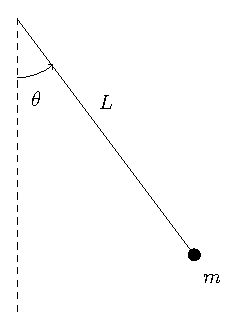
\includegraphics[scale=1.3]{Imagenes/pendulo_01.eps}
    \caption{Péndulo simple.}
\end{figure}
Las fuerzas que actúan sobre la masa $m$, son la tensión $T$ de la cuerda y el peso $mg$; usando la segunda ley de Newton, tenemos que
\begin{align}
\text{Centrípeta} \hspace{0.5cm} T - m \, g \, \cos \theta &= \dfrac{m \, v^{2}}{L}  \label{eq:ecuacion_pendulo_01} \\
\text{Tangencial} \hspace{0.5cm} -m \, g \, \sin \theta &= m \dv[2]{t} (L \, \theta) \label{eq:ecuacion_pendulo_02}
\end{align}
Considerando la ecuación tangencial (\ref{eq:ecuacion_pendulo_02}) y luego de acomodar términos, tenemos que
\begin{equation} \dv[2]{\theta}{t} + \dfrac{g}{L} \, \sin \theta = 0
\label{eq:ecuacion_pendulo_03}
\end{equation}
La aproximación usual para oscilaciones de pequeña amplitud es tomar el término principal en la expansión de la serie del seno, en cuyo caso el movimiento descrito es el de un oscilador armónico simple y el período es
\begin{align*}
T = 2 \, \pi \,\sqrt{\dfrac{L}{g}}
\end{align*}
\par
Para obtener una solución exacta de la ec. (\ref{eq:ecuacion_pendulo_03}), se multiplica por $\displaystyle{\dv{\theta}{t}}$, para obtener
\begin{equation}
\dv{t} \left[ \dfrac{1}{2} \, \left( \dv{\theta}{t} \right)^{2} - \dfrac{g}{L} \, \cos \theta \right] = 0
\label{eq:ecuacion_pendulo_04}
\end{equation}
La ecuación anterior nos dice que la cantidad entre los corchetes es una constante\footnote{De hecho, si multiplicamos por $m \, L^{2}$, vemos que el primer término es la energía cinética y el segundo es la energía potencial gravitatoria. La ecuación comprueba entonces el teorema de conservación de energía.}. Para obtener el valor de la constante, suponemos que liberamos el péndulo del reposo, por lo que el péndulo se desplaza del ángulo $\theta$ a $\theta_{0}$, esto nos conduce a
\begin{align*}
\dv{\theta}{t} = \sqrt{\dfrac{2 \, g}{L} \, (\cos \theta - \cos \theta_{0})}
\end{align*}
Podemos utilizar la siguiente identidad trigonométrica $\cos 2 \, x = 1 - 2 \, \sin^{2} x$, para entonces ordenar los términos de la ecuación, con lo cual
\begin{align*}
2 \, \sqrt{\dfrac{g}{L}} \int \, \dd{t} = \int \dfrac{\dd{\theta}}{[k^{2} - \sin^{2} (\theta/2)]^{1/2}}
\end{align*}
En la integral, $k = \sin (\theta_{0}/2)$. Como el ángulo $\theta \leq \theta_{0}$, podemos hacer el cambio de variable $\sin \phi = k^{-1} \, \sin (\theta/2)$, para entonces obtener
\begin{align*}
\sqrt{\dfrac{g}{L}} \int \, \dd{t} = \int \dfrac{\dd{\phi}}{\sqrt{1 - k^{2} - \sin^{2} \phi}}
\end{align*}
La integral de la derecha es una \emph{interal elíptica de primera clase}, descrita por
\begin{align*}
F(k , \phi) = \int_{0}^{\phi} \dfrac{\dd{\phi^{\prime}}}{\sqrt{1 - k^{2} \, \sin^{2} \phi^{\prime} }}
\end{align*}
El tiempo necesario para que el ángulo cambie de $0$ a $\theta_{0}$ es un cuarto del período $T$. En este tiempo, el ángulo $\phi$ cambia de $0$ a $\pi/2$. Con esos límites, se tiene que la integral es
\begin{equation}
F(k) = \int_{0}^{\pi/2} \dfrac{\dd \phi}{\sqrt{1 - k^{2} \, \sin^{2} \phi} }
\label{eq:ecuacion_pendulo_05}
\end{equation}
y se le conoce como la \emph{integral elíptica completa} de primera clase.
\par
Utilizando el resultado que expresa una serie
\begin{equation}
(1 - z)^{s} = \sum_{k=0}^{\infty} \dfrac{(-s)_{k}}{k!} \, z^{k}
\label{eq:ecuacion_pendulo_06}
\end{equation}
Para evaluar la integral $F(k)$, usamos el resultado de la ec. (\ref{eq:ecuacion_pendulo_06}) para expandir el integrando
\begin{align*}
[ 1 - k^{2} \, \sin^{2} \phi ]^{-1/2} = \sum_{n=0}^{\infty} \dfrac{(\frac{1}{2})_{n}}{n!} \, k^{2 n} \, \sin^{2 n} \phi
\end{align*}
Al sustituir esta expansión en la ec. (\ref{eq:ecuacion_pendulo_05}) es posible evaluar una integral del tipo
\begin{align*}
\int \sin^{p} \, x \, \dd{x} = \int \sin^{2 n} \, \phi \, \dd{\phi}
\end{align*}
Integrando por partes
\begin{align*}
\int \sin^{p} \, x \, \dd{x} &= - \sin^{p-1} \, x \, \cos x + (p - 1) \, \int \sin^{p-1} \, x \, \cos^{2} \, x \, \dd{x} \\
&= -\sin^{p-1} x \, \cos x + (p - 1) \, \int \sin^{p-2} x \, \dd{x} - (p - 1) \, \int \sin^{p} x \dd{x} 
\end{align*}
Resolviendo para $\displaystyle{\int \sin^{p} x \, \dd{x}}$, llegamos a la fórmula
\begin{align*}
\int \sin^{p} x \, \dd{x} = - \dfrac{\sin^{p-1} \, x \, \cos x}{p} + \dfrac{p - 1}{p} \int \sin^{p-2} x \, \dd{x}
\end{align*}
Ocupando la fórmula nuevamente en la integral de la derecha, se tiene que
\begin{align*}
\int \sin^{p} x \, \dd{x} &= - \dfrac{\sin^{p-1} \, x \, \cos x}{p} + \dfrac{p - 1}{p} \, \dfrac{\sin^{p-3} \, x \, \cos x}{(p - 2)} + \\
&+ \dfrac{(p - 1)(p - 3)}{p \, (p - 2)} \int \sin^{p-4} \, x \, \dd{x}
\end{align*}
Repitiendo el uso de la fórmula siempre se tendrá como resultado una suma de términos, cada uno de los cuales involucra un producto del $\cos x$ con alguna de potencia del $\sin x$, más una integral con una potencia de $\sin x$. Si tomamos el rango de integración de $0$ a $\pi / 2$, entonces el $\cos x$ se anula en un límite y $\sin x$ se anula en el otro. Sólo el término con la integral permanece. El resultado es entonces
\begin{align*}
&\int_{0}^{\pi/2} \sin^{p} \, x \, \dd{x} = \\
&= \begin{dcases}
\dfrac{(p-1)(p-3) \ldots (p - (p-1))}{p(p-2) \ldots (p -(p-2))} \int_{0}^{\pi/2} \, \dd{x},  & p = 0, 2, 4, \ldots \\[1em]
\dfrac{(p-1)(p-3) \ldots (p - (p-2))}{p(p-2) \ldots (p -(p-3))} \int_{0}^{\pi/2} \sin x \, \dd{x}, & p = 1, 3, 5, \ldots
\end{dcases}
\end{align*}
Las integrales de la derecha se pueden evaluar directamente para obtener $\pi/2$ y $1$, respectivamente. La notación más compacta de Pochhammer para los productos queda expresada como
\begin{align*}
\int_{0}^{\pi/2} \sin^{p} x \, \dd{x} = \begin{cases}
\dfrac{\pi}{2} \, \dfrac{\left( 1/2 \right)_{p/2}}{(p/2)!}, & p = 0, 2, 4, \ldots \\[1em]
\dfrac{((p-1)/2)!}{(3/2)_{(p-1)/2}}. & p = 1, 3, 5, \ldots
\end{cases}
\end{align*}
Si el resultado para valores pares de $p$ se incluyen en la expansión del integrando en la ecuación (\ref{eq:ecuacion_pendulo_05}), la integral elíptica completa es
\begin{align*}
F(k) &= \dfrac{\pi}{2} \sum_{n=0}^{\infty} \dfrac{\left(\frac{1}{2} \right)_{n} \, \left(\frac{1}{2} \right)_{n}}{n! \, (1)_{n}} \, k^{2n} \\[0.5em]
&= \dfrac{\pi}{2} \, {}_{2} F_{1} \left( \dfrac{1}{2}, \dfrac{1}{2}, 1; k^{2} \right)
\end{align*}
Nota: observamos que también es común denotar la función hipergeométrica por ${}_{2} F_{1} (a, b, c; x)$. Esta notación de aspecto ligeramente extraño significa que, en el coeficiente de cada potencia de $x$, hay dos parámetros ($a$ y $b$) en el numerador y un parámetro ($c$) en el denominador.
\par
Así, el período de oscilación de un péndulo simple está dado por
\begin{align*}
T = 2 \, \pi \, \sqrt{\dfrac{L}{g}} \, {}_{2} F_{1} \left(\frac{1}{2}, \frac{1}{2}, 1; \sin^{2} \left( \dfrac{\theta_{0}}{2} \right) \right)
\end{align*}
Claramente, el período depende de la amplitud de la oscilación. Sin embargo, si la amplitud es pequeña, podemos usar sólo el término principal en las series hipergeométricas. Entonces, el período se reduce a la aproximación habitual de ángulo pequeño:
\begin{align*}
T = 2 \, \pi (L / g)^{1/2} \hspace{2cm} \theta_{0} \ll 1
\end{align*}
La integral elíptica de segunda clase está definida por
\begin{align*}
E (k, \phi) = \int_{0}^{\phi} \sqrt{1 - k^{2} \, \sin^{2} \phi^{\prime}} \, \dd{\phi^{\prime}}
\end{align*}
La integral elíptica completa de segunda clase se relaciona con la función hipergeométrica por
\begin{equation}
E(k) = \int_{0}^{\pi/2} \sqrt{1 - k^{2} \, \sin^{2} \phi} \, \dd{\phi} =  \dfrac{\pi}{2} \, F \left( -\dfrac{1}{2}, \dfrac{1}{2}, 1; k^{2} \right)
\end{equation}
\end{document}